\chapter{Implementation}
\label{implementation}
This chapter details on the implementation of the concepts discussed in previous chapter for route planner and trajectory planner modules. All the modules are implemented as independent nodes in Robot Operating System (ROS) and communicate with each other using ROS messages.

\begin{figure}
	\centering
	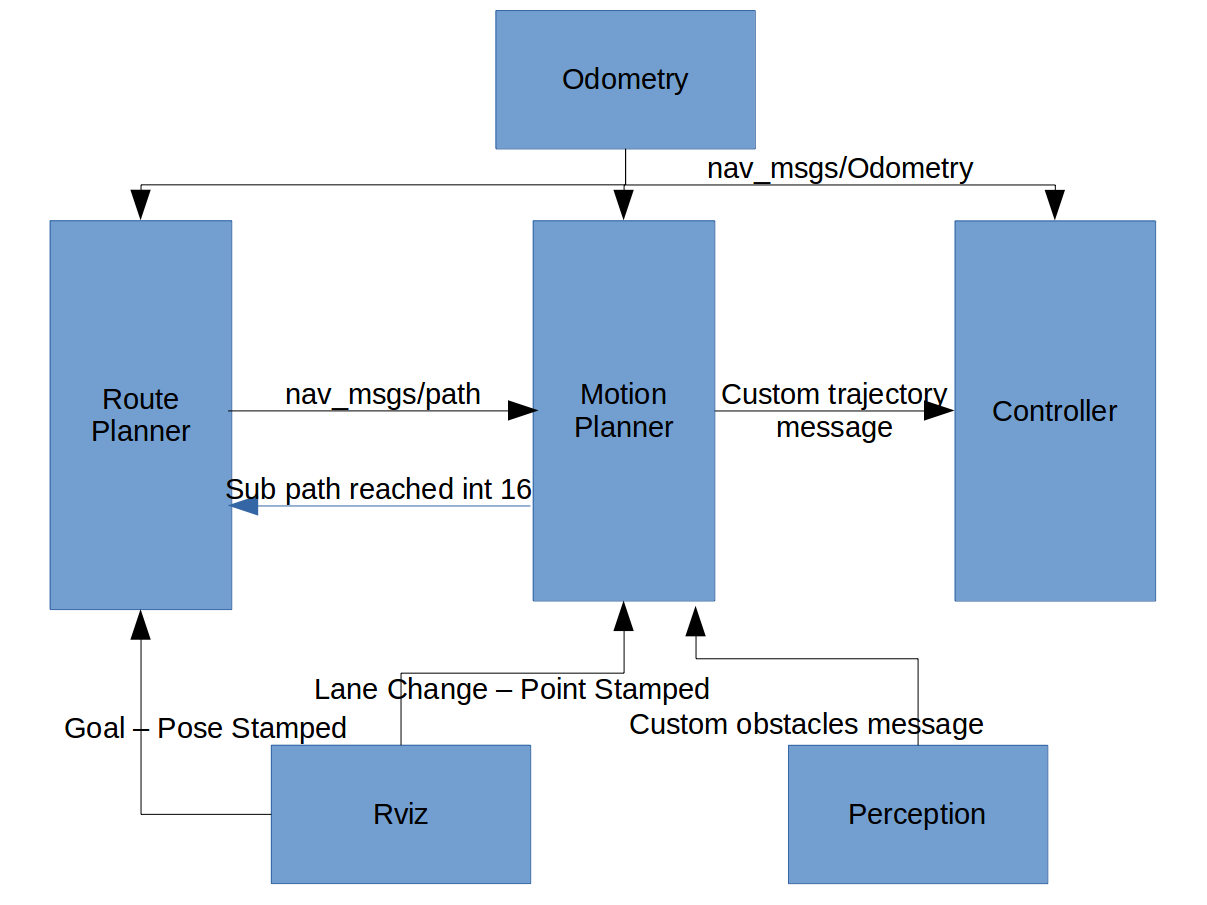
\includegraphics[width=0.9\textwidth]{Images/implementation/message_flow.png}
	\caption{Message Flow across Modules}
	\label{message_flow}
\end{figure}


\section{Route Planner}
Route planner parses the RNDF file and stores way points, their relation to lanes and further to segments. The below code segment shows the declaration of the way point, here coordi indicates the coordinates of way points, idn is the unique id for each way point and parent is the lane to which way point belongs. Similarly there lane stores set of way points, parent is the segment to which the lane belongs. 

\begin{lstlisting}
class c_waypoint(object):
	def __init__(self,name,coordi,parent, idn):
		self.name = name
		self.coordi = coordi
		self.parent = parent
		self.idn = idn
	def __str__(self):
		return '{}'.format(self.name)

\end{lstlisting}



\begin{figure}
	\centering
	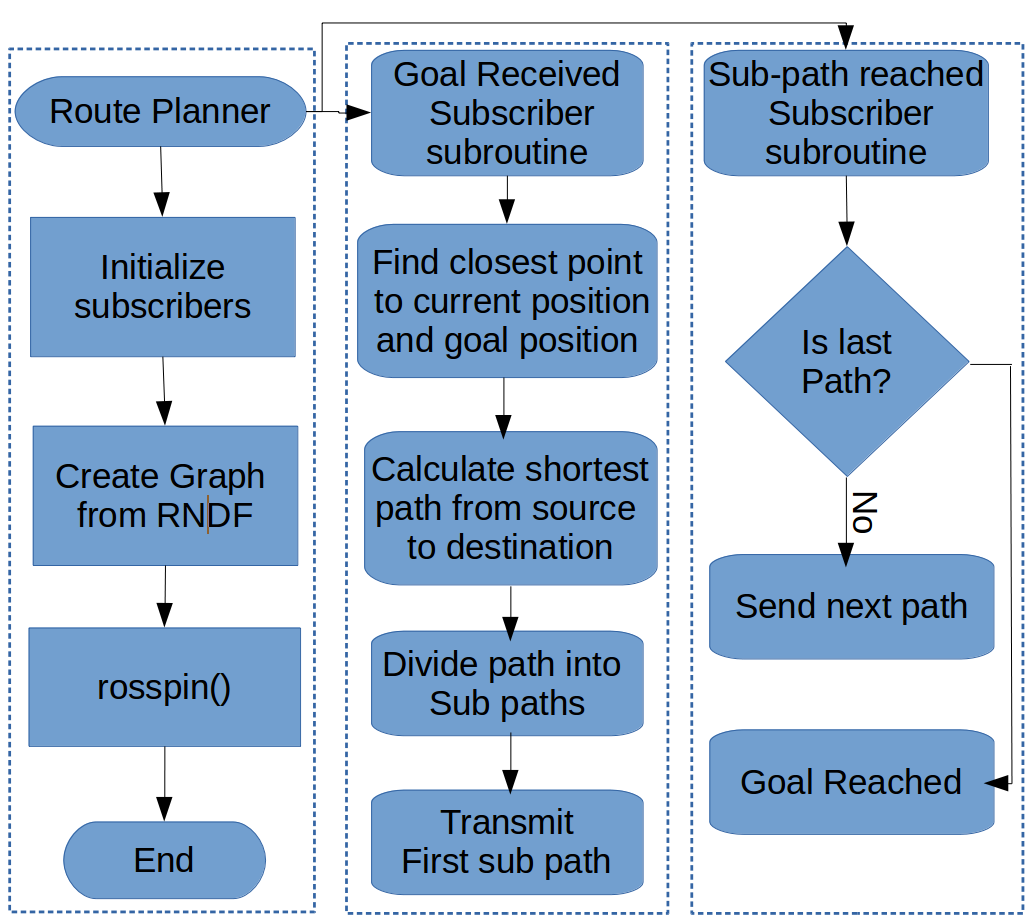
\includegraphics[width=0.8\textwidth]{Images/implementation/route_planner.png}
	\caption{Route Planner Functions}
	\label{route_planner_func}
\end{figure}

\section{Motion Planner}

\begin{figure}
	\centering
	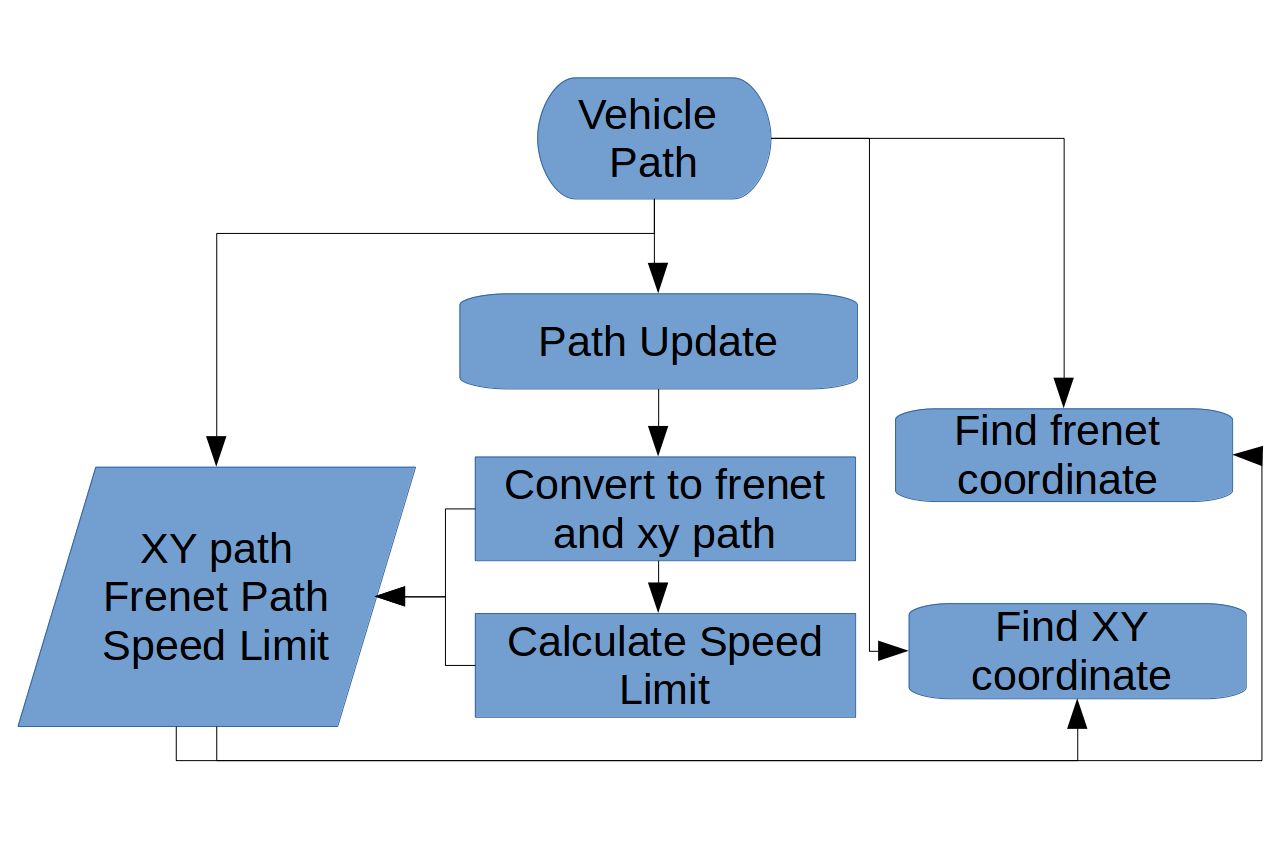
\includegraphics[width=0.8\textwidth]{Images/implementation/vehicle_path.png}
	\caption{Vehicle Path Class}
	\label{vehicle_path_class}
\end{figure}

\begin{figure}
	\centering
	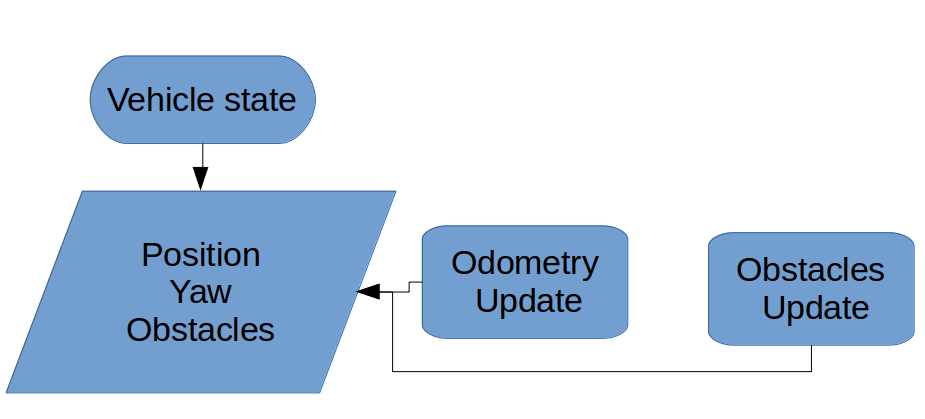
\includegraphics[width=0.8\textwidth]{Images/implementation/vehicle_state.png}
	\caption{Vehicle State Class}
	\label{vehicle_state_class}
\end{figure}

\begin{figure}
	\centering
	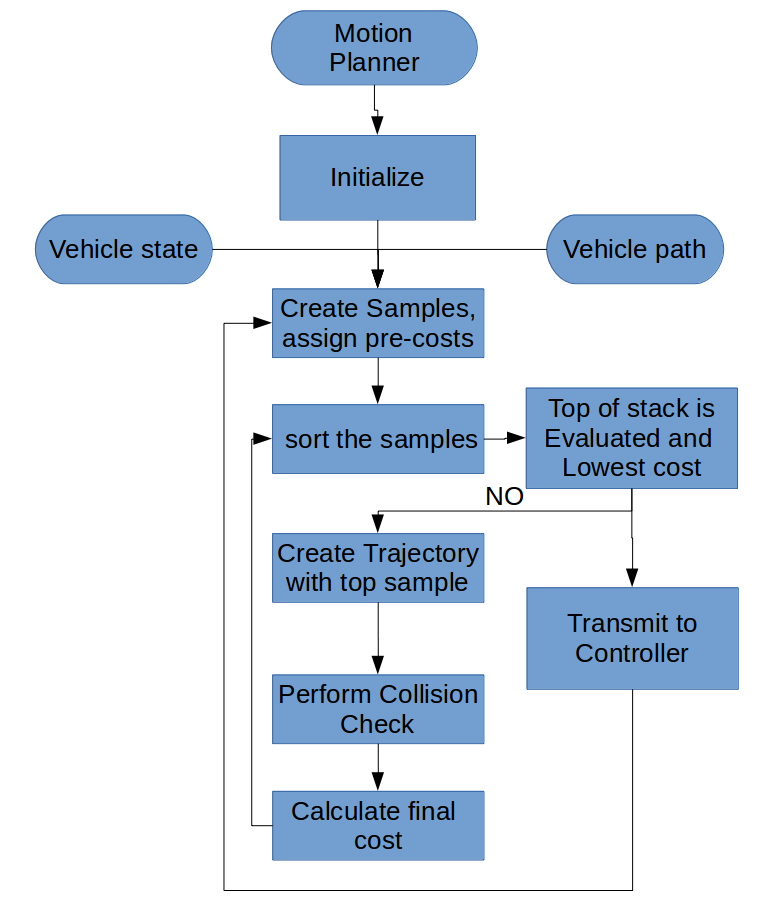
\includegraphics[width=0.8\textwidth]{Images/implementation/motion_planner.png}
	\caption{Motion Planner Functions}
	\label{motion_planner_func}
\end{figure}






\iffalse

Code for storing 

class c_exit(object):
def __init__(self, entry, exit, parent):
self.entry = entry
self.exit = exit
self.parent = parent

class c_lane(object):
def __init__(self,name,parent,idn):
self.name = name
self.parent = parent
self.idn = idn
self.waypoints = []
self.exits = []
def add_waypoint(self,waypoint):
self.waypoints.append(waypoint)
def add_exit(self,exit):
self.exits.append(exit)
def __str__(self):
return '{}'.format(self.name)

class c_segment(object):
def __init__(self,name,parent,idn):
self.name = name
self.lanes = []
self.parent = parent
self.idn = idn
def add_lane(self,lane):
self.lanes.append(lane)
def __str__(self):
return '{}'.format(self.name)

class c_rndf(object):
def __init__(self,name):
self.name = name
self.segments= []
def add_segment(self,segment):
self.segments.append(segment)
def __str__(self):
return '{}'.format(self.name)
Check if this chapter is needed, 

Write a flow chart describing various functions implemented 

How the collision check is implemented

Further details on how these trajectories are converted to x,y coordinates used by the trajectory follower and the constraints in implementation for model car will be discussed in

How costs are added

Which messages are used for what, who sends what and who receives what - flow diagrams

speak about splines, how the state machine works, write a flowchart etc

Inform when which order splines are good to implemented

need for adding extra costs if this has to be ported for full scale cars

Issues - 
\fi